General Relativity and the Standard Model of Particle Physics (a quantum field theory) have been incredibly successful at explaining physics at very long and short distance scales. However, it has been known for over a century that a fundamentally quantum mechanical description of gravity requires a drastic paradigm shift. The need for a theory of gravity is not just for aesthetics' sake but is fundamentally necessary to understand the physics of black holes and early cosmology.

\begin{figure}[H]
  \centering
  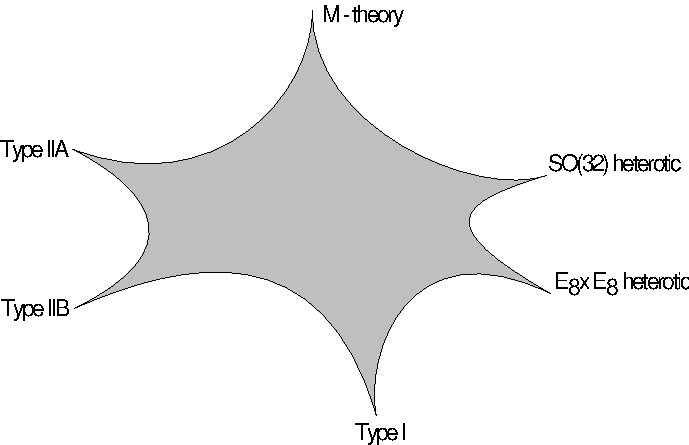
\includegraphics{external/superstring-theories}
  \caption{Various flavors of perturbative string theory as cusps of this diagram related by string dualities in appropriate limits (taken from \cite{Polchinski:1999br})}
  \label{fig:superstring-theories}
\end{figure}

It is common knowledge now that string theory provides a concrete realization of quantum gravity without any inconsistencies or divergences. String theory started its life as worldsheet perturbation theory. However, today, we understand that non-perturbative aspects of string theory, particularly various dualities that relate seemingly different superstring theories, play a crucial role in the subject. The discovery of these dualities led to the famous picture of \cref{fig:superstring-theories} taken from \cite{Polchinski:1999br}. Superstring theories should be thought of as asymptotic expansions around the cusps of this diagram. The description of physics in the "bulk" (finite distance away from the cusps) still eludes us.

One of the most outstanding consequences of string dualities is the gauge-gravity correspondence \cite{Susskind:1994vu,Maldacena:1997re}. The duality relates a gauge theory in $d$ dimensional spacetime to quantum gravity (string theory) in $d+1$ dimensions, where the $d$ dimensional spacetime is interpreted as the boundary of the $d+1$ dimensional bulk theory. It is a consequence of the open-closed string duality. See \cite{Aharony:1999ti, Witten:1998qj} for excellent reviews of the conjecture. Many explicit examples of holographic correspondence have been found over the years, and the correspondence has been explicitly proved in certain situations \cite{Eberhardt:2019ywk,Gaberdiel:2021qbb}. 

Gauge-gravity duality has been instrumental in understanding gauge theories and gravitational physics (i.e., black holes). It is an example of weak-strong duality, meaning that strongly coupled physics of gauge theories can be understood from weakly coupled gravity, where stringy corrections can be ignored. E.g., AdS/QCD is a theoretical framework that uses the gauge-gravity correspondence as a tool to study strongly coupled color physics of hadrons and baryons \cite{Casalderrey-Solana:2011dxg,Kim:2012ey}; AdS/CMT, a developing field, uses the duality to study complex condensed matter systems such as non-Fermi liquids and strongly correlated electrons and aspects of quantum criticality, and quantum entanglement in such systems \cite{Sachdev:2010ch,Jensen:2010em}. The utility of the duality goes both ways. Recently, it was used to compute the rate of Hawking evaporation of AdS black holes, the so-called Page curve \cite{Almheiri_2020,Gautason:2020tmk,Cadoni:2021ypx}. A very accessible introduction to AdS/CFT is given in \cite{Pinaki}.

Matrix models are gauge theories in $0+1$ dimensions (i.e., quantum mechanics) that are amenable to a dual gravity description. The BFSS Matrix model was conjectured by T. Banks, W. Fischler, S. H. Shenker, and L. Susskind \cite{Banks:1996vh} to reproduce the S-matrix of 11-dimensional M-theory in certain limits. In particular, at low energies, M-theory reduces to the 11-dimensional Supergravity of E. Cremmer, B. Julia, and J. Scherk \cite{Cremmer:1978km}.

\section{Motivation}

One obtains two kinds of asymptotic expansions starting from Type IIA superstring theory. The string theory has two parameters, $\alpha' \propto \ell_s^2$ related to the string tension and length ($\ell_s$), and the string coupling constant $g_s$ that controls the contributions of worldsheets of various topologies. The string perturbation series at the lowest order in $\alpha'$ reproduces supergravity equations of motion. $\alpha'$ corrections represent stringy higher derivative corrections to the ordinary supergravity action. The $10$-dimensional Plack length $\ell_p$ (or equivalently, Newton's constant $G_N$) is related to the string coupling $g_s$. 

In a gauge theory, however, the important parameter is the 't Hooft coupling $\lambda$ related to the Yang-Mills coupling $g_{\mathrm{YM}}$ as $\lambda = g_\mathrm{YM}^2 N$ where $N$ is the rank of the gauge group $\mathrm{U}(N)$. In holographic duality, one can show that parameters on one side are related to those on the other as follows
\begin{align}\label{eqn:duality-parameters}
  \frac{R_\mathrm{eff}^2}{\alpha'} &\sim \sqrt{\frac{\lambda}{r^3}} \\
  g_s &\sim \frac{\ell_p^4}{\ell_s^4} \sim \frac{\lambda}{N}
\end{align}

The first relation says that the effective radius of curvature measured in units of string length corresponds directly to the 't Hooft coupling (and the radial coordinate in the bulk $r$). Thus, in the regime where the radius of curvature is much larger than the string length (and we can trust ordinary supergravity without stringy corrections), the 't Hooft coupling is big, and the gauge theory is strongly coupled. Secondly, at fixed $\lambda$, taking a large $N$ limit corresponds to taking $\ell_p \to 0$, in other words, ignoring quantum gravity corrections. This is precisely the regime where classical supergravity calculations hold!

Note that the 't Hooft coupling $\lambda$ has dimensions of $(\mathrm{energy})^3$; thus, low energies correspond to strong coupling and high energies to weak coupling. Further, due to \cref{eqn:duality-parameters}, the dual bulk geometry is highly curved near the boundary $r \to \infty$ and stringy corrections cannot be ignored. This is summarized in \cref{fig:boundary} taken from \cite{Maldacena:2018vsr}.

\begin{figure}[H]
  \centering
  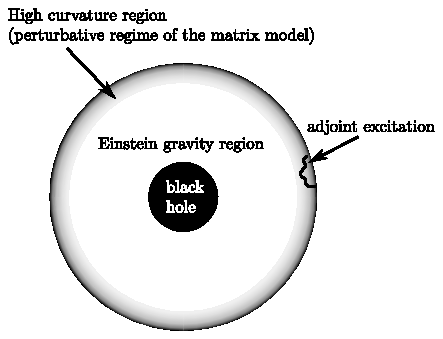
\includegraphics{external/boundary}
  \caption{A schematic picture of the bulk geometry arising through the holographic correspondence. The boundary region is highly stringy, whereas classical gravity can be trusted in the deep bulk.}
  \label{fig:boundary}
\end{figure}

In this dissertation, we study the opposite limit, namely, the limit of large energies and hence of weak coupling in the matrix theory. This enables us also to take the classical limit and ignore quantum corrections to the leading order. Despite dropping quantum corrections, we find results reminiscent of black hole physics. Note that in this limit, the dual gravity picture is highly stringy, and in essence, we are attempting to explore near the boundary region of \cref{fig:boundary}.


\section{Outline}

In the next chapter, we will go through a quick review of the BFSS matrix model to set up notation and define the observables we study. In Chapter 3, we summarize our results: Section 3.2 demonstrates the precise nature of chaos in Matrix theory and the lessons to be learned from it. Section 3.3 highlights independence from initial conditions of the time statistics of various observables. Moreover, the last two sections talk about connections with random matrix theory. By comparing simulations with random matrix ensembles, we find that over long times and at large $N$, matrix model dynamics fit a random Gaussian Unitary ensemble (GUE) surprisingly well. We suggest and study various estimates for the parameters of this emergent random matrix ensemble. In the last section, we take note of the universal properties of matrix theory that depart from this random matrix behavior. The results presented in this chapter suggest the following picture of black hole microstates (see \cite{Susskind:1993ws,Horowitz:1996nw}):

\textit{
  Random, time-dependent states (of D0-branes and strings stretching between them) in matrix theory mimic black hole microstates in the underlying quantum gravity.
}

The fuzzball program \cite{Mathur:2005zp} is a similar attempt to parametrize the set of black hole microstates as fuzzball geometries which are highly stringy geometries without a horizon. The fuzzball proposal has lately been a subject of intense discussion and critique (see, e.g., \cite{Raju:2018xue}).
  
Finally, we end this dissertation by discussing our results, plans for the future, and open questions.